\documentclass[a4paper,10pt]{book}
\usepackage[utf8]{inputenc}
\usepackage{fullpage}
\usepackage{cite}
\usepackage[utf8]{inputenc}
\usepackage{a4wide}
\usepackage{url}
\usepackage{graphicx}
\usepackage{caption}
\usepackage{float} % para que los gr\'aficos se queden en su lugar con [H]
\usepackage{subcaption}
\usepackage{wrapfig}
\usepackage{color}
\usepackage{amsmath} %para escribir funci\'on partida , matrices
\usepackage{amsthm} %para numerar definciones y teoremas
\usepackage[hidelinks]{hyperref} % para inlcuir links dentro del texto
\usepackage{tabu} 
\usepackage{comment}
\usepackage{amsfonts} % \mathbb{N} -> conjunto de los n\'umeros naturales  
\usepackage{enumerate}
\usepackage{listings}
\usepackage[colorinlistoftodos, textsize=small]{todonotes} % Para poner notas en el medio del texto!! No olvidar hacer. 
\usepackage{framed} % Para encuadrar texto. \begin{framed}
\usepackage{csquotes} % Para citar texto \begin{displayquote}
\usepackage{epigraph} % Epigrafe  \epigraph{texto}{\textit{autor}}
\usepackage{authblk}
\usepackage{titlesec}
\usepackage{varioref}
\usepackage{bm} % \bm{\alpha} bold greek symbol
\usepackage{pdfpages} % \includepdf
\usepackage[makeroom]{cancel} % \cancel{} \bcancel{} etc
\usepackage{wrapfig} % \begin{wrapfigure} Pone figura al lado del texto
\usepackage{mdframed}
\usepackage{algorithm}
%\usepackage{quoting}
\usepackage{mathtools}	
\usepackage{tikz}
\usepackage{paracol}

\newcommand{\vm}[1]{\mathbf{#1}}
\newcommand{\N}{\mathcal{N}}
\newcommand{\citel}[1]{\cite{#1}\label{#1}}
\newcommand\hfrac[2]{\genfrac{}{}{0pt}{}{#1}{#2}} %\frac{}{} sin la linea del medio

\newtheorem{midef}{Definition}
\newtheorem{miteo}{Theorem}
\newtheorem{mipropo}{Proposition}

\theoremstyle{definition}
\newtheorem{definition}{Definition}[section]
\newtheorem{theorem}{Theorem}[section]
\newtheorem{proposition}{Proposition}[section]


%http://latexcolor.com/
\definecolor{azul}{rgb}{0.36, 0.54, 0.66}
\definecolor{rojo}{rgb}{0.7, 0.2, 0.116}
\definecolor{rojopiso}{rgb}{0.8, 0.25, 0.17}
\definecolor{verdeingles}{rgb}{0.12, 0.5, 0.17}
\definecolor{ubuntu}{rgb}{0.44, 0.16, 0.39}
\definecolor{debian}{rgb}{0.84, 0.04, 0.33}
\definecolor{dkgreen}{rgb}{0,0.6,0}
\definecolor{gray}{rgb}{0.5,0.5,0.5}
\definecolor{mauve}{rgb}{0.58,0,0.82}

\lstset{
  language=Python,
  aboveskip=3mm,
  belowskip=3mm,
  showstringspaces=true,
  columns=flexible,
  basicstyle={\small\ttfamily},
  numbers=none,
  numberstyle=\tiny\color{gray},
  keywordstyle=\color{blue},
  commentstyle=\color{dkgreen},
  stringstyle=\color{mauve},
  breaklines=true,
  breakatwhitespace=true,
  tabsize=4
}

% tikzlibrary.code.tex
%
% Copyright 2010-2011 by Laura Dietz
% Copyright 2012 by Jaakko Luttinen
%
% This file may be distributed and/or modified
%
% 1. under the LaTeX Project Public License and/or
% 2. under the GNU General Public License.
%
% See the files LICENSE_LPPL and LICENSE_GPL for more details.

% Load other libraries

%\newcommand{\vast}{\bBigg@{2.5}}
% newcommand{\Vast}{\bBigg@{14.5}}
% \usepackage{helvet}
% \renewcommand{\familydefault}{\sfdefault}

\usetikzlibrary{shapes}
\usetikzlibrary{fit}
\usetikzlibrary{chains}
\usetikzlibrary{arrows}

% Latent node
\tikzstyle{latent} = [circle,fill=white,draw=black,inner sep=1pt,
minimum size=20pt, font=\fontsize{10}{10}\selectfont, node distance=1]
% Observed node
\tikzstyle{obs} = [latent,fill=gray!25]
% Invisible node
\tikzstyle{invisible} = [latent,minimum size=0pt,color=white, opacity=0, node distance=0]
% Constant node
\tikzstyle{const} = [rectangle, inner sep=0pt, node distance=0.1]
%state
\tikzstyle{estado} = [latent,minimum size=8pt,node distance=0.4]
%action
\tikzstyle{accion} =[latent,circle,minimum size=5pt,fill=black,node distance=0.4]
\tikzstyle{fijo} =[latent,circle,minimum size=5pt,fill=black]


% Factor node
\tikzstyle{factor} = [rectangle, fill=black,minimum size=10pt, draw=black, inner
sep=0pt, node distance=1]
% Deterministic node
\tikzstyle{det} = [latent, rectangle]

% Plate node
\tikzstyle{plate} = [draw, rectangle, rounded corners, fit=#1]
% Invisible wrapper node
\tikzstyle{wrap} = [inner sep=0pt, fit=#1]
% Gate
\tikzstyle{gate} = [draw, rectangle, dashed, fit=#1]

% Caption node
\tikzstyle{caption} = [font=\footnotesize, node distance=0] %
\tikzstyle{plate caption} = [caption, node distance=0, inner sep=0pt,
below left=5pt and 0pt of #1.south east] %
\tikzstyle{factor caption} = [caption] %
\tikzstyle{every label} += [caption] %

\tikzset{>={triangle 45}}

%\pgfdeclarelayer{b}
%\pgfdeclarelayer{f}
%\pgfsetlayers{b,main,f}

% \factoredge [options] {inputs} {factors} {outputs}
\newcommand{\factoredge}[4][]{ %
  % Connect all nodes #2 to all nodes #4 via all factors #3.
  \foreach \f in {#3} { %
    \foreach \x in {#2} { %
      \path (\x) edge[-,#1] (\f) ; %
      %\draw[-,#1] (\x) edge[-] (\f) ; %
    } ;
    \foreach \y in {#4} { %
      \path (\f) edge[->,#1] (\y) ; %
      %\draw[->,#1] (\f) -- (\y) ; %
    } ;
  } ;
}

% \edge [options] {inputs} {outputs}
\newcommand{\edge}[3][]{ %
  % Connect all nodes #2 to all nodes #3.
  \foreach \x in {#2} { %
    \foreach \y in {#3} { %
      \path (\x) edge [->,#1] (\y) ;%
      %\draw[->,#1] (\x) -- (\y) ;%
    } ;
  } ;
}

% \factor [options] {name} {caption} {inputs} {outputs}
\newcommand{\factor}[5][]{ %
  % Draw the factor node. Use alias to allow empty names.
  \node[factor, label={[name=#2-caption]#3}, name=#2, #1,
  alias=#2-alias] {} ; %
  % Connect all inputs to outputs via this factor
  \factoredge {#4} {#2-alias} {#5} ; %
}

% \plate [options] {name} {fitlist} {caption}
\newcommand{\plate}[4][]{ %
  \node[wrap=#3] (#2-wrap) {}; %
  \node[plate caption=#2-wrap] (#2-caption) {#4}; %
  \node[plate=(#2-wrap)(#2-caption), #1] (#2) {}; %
}

% \gate [options] {name} {fitlist} {inputs}
\newcommand{\gate}[4][]{ %
  \node[gate=#3, name=#2, #1, alias=#2-alias] {}; %
  \foreach \x in {#4} { %
    \draw [-*,thick] (\x) -- (#2-alias); %
  } ;%
}

% \vgate {name} {fitlist-left} {caption-left} {fitlist-right}
% {caption-right} {inputs}
\newcommand{\vgate}[6]{ %
  % Wrap the left and right parts
  \node[wrap=#2] (#1-left) {}; %
  \node[wrap=#4] (#1-right) {}; %
  % Draw the gate
  \node[gate=(#1-left)(#1-right)] (#1) {}; %
  % Add captions
  \node[caption, below left=of #1.north ] (#1-left-caption)
  {#3}; %
  \node[caption, below right=of #1.north ] (#1-right-caption)
  {#5}; %
  % Draw middle separation
  \draw [-, dashed] (#1.north) -- (#1.south); %
  % Draw inputs
  \foreach \x in {#6} { %
    \draw [-*,thick] (\x) -- (#1); %
  } ;%
}

% \hgate {name} {fitlist-top} {caption-top} {fitlist-bottom}
% {caption-bottom} {inputs}
\newcommand{\hgate}[6]{ %
  % Wrap the left and right parts
  \node[wrap=#2] (#1-top) {}; %
  \node[wrap=#4] (#1-bottom) {}; %
  % Draw the gate
  \node[gate=(#1-top)(#1-bottom)] (#1) {}; %
  % Add captions
  \node[caption, above right=of #1.west ] (#1-top-caption)
  {#3}; %
  \node[caption, below right=of #1.west ] (#1-bottom-caption)
  {#5}; %
  % Draw middle separation
  \draw [-, dashed] (#1.west) -- (#1.east); %
  % Draw inputs
  \foreach \x in {#6} { %
    \draw [-*,thick] (\x) -- (#1); %
  } ;%
}


\usepackage{physics}
\newcommand*\diff{\mathop{}\!\mathrm{d}}

\newif\ifen
\newif\ifes
\newcommand{\en}[1]{\ifen#1\fi}
\newcommand{\es}[1]{\ifes#1\fi}
\estrue


%opening
\title{\huge Inferencia y evolución cultural}
\author{Gustavo Landfried}

\begin{document}

\maketitle

\tableofcontents

\chapter{Conocimiento empírico}

La ciencia es una institución humana que tiene pretención de verdad, de formular proposiciones que valgan para todas las personas, tanto intercultural como intersubjetivamente.
Las ciencias formales validan sus proposiciones mediante teoremas, resultados derivados de aplicar las reglas internas a un sistema axiomático cerrado.
Las ciencias empíricas deben validar sus proposiciones dentro de sistemas abiertos, lo que impone siempre un grado de incertidumbre asociada.
¿Cuál es entonces la fuente de validez del conocimiento empírico?

\section{Vida}

En el último tercio de la historia del Universo, en algún momento hace aproximadamente 4500 millones de años, apareció en la tierra una forma de organización de la materia capaz de auto-replicarse.
El crecimiento de estos linajes siguieron procesos multiplicativos y ruidosos: secuencias de probabilidades de supervivencia y reproducción.
Los errores producidos durante la replicación diversificaron las formas de organización de la materia, y las diferentes tazas de superviencia favorecieron a aquellas mejor adaptadas al medio.
Las diversas formas que adquiere la vida constituyen conocimiento empíricamente válido en tanto que contiene información que es capaz de interectuar con el medio y sobrevivir.
En este sentido, ``la vida'' puede ser vista como un sistema natural de validación distribuida de información empírica.

% Parrafo

La complejidad actual de la vida~\cite{barOn2018-biomass} es consecuencia de una serie de transiciones evolutivas~\cite{maynardSmith1995-majorTransitions} en las que las entidades, que antes eran capaces de replicarse de forma independiente, luego de la transición pasan a replicarse sólo como partes de una unidad mayor.
La tabla~\ref{tab:transitions} enumera algunas de las principales transiciones ocurridas en la historia evolutiva de la vida.
\begin{table}[ht!] \centering
    \begin{tabular}{l}
        \hline
        \es{De moléculas a poblaciones de moléculas}
        \\%        
        \es{De células procariotas a eucariotas}
        \\%
        \es{De clones asexuales a poblaciones sexuales}
        \\%
        \es{De entidades unicelulares a multicelulares}
        \\%
        \es{De individuos a sociedades}
        \\
        \hline
    \end{tabular}
    \caption{
    \es{Algunas de la principales transiciones evolutivas}
    }
    \label{tab:transitions}
\end{table}
Los saltos en los niveles de complejidad traen consigo la aparición de formas de ``división social del trabajo'' al interior de las poblaciones (e.g. diferenciación funcional de las células en organismos multicelulares), y cambios en el almacenamiento y transmisión de información (e.g. los sistemas de información cultural en las especies sociales).

% Parrafo

Hasta hace poco se consideró una verdad establecida que la cooperación requería algún tipo de comportamiento altruista para evolucionar.
Esta conclusión supone implícitamente que los procesos evolutivos son ergódicos.
Decimos que un proceso es ergódico si la media temporal de una transformación $f(\cdot)$ de los estados del sistema es igual al su valor esperado,
\begin{equation}
 \underbrace{\lim_{T \mapsto \infty} \int_0^T f(\omega(t)) \diff t}_{\text{Media temporal}}  = \underbrace{\int_{\Omega} f(\omega)p(\omega) \diff\omega}_{\text{Valor esperado}}
\end{equation}
donde $\omega \in \Omega$ representa los estados del sistema, $\omega(t)$ el estado del sistema obtenido aleatoriamente en el tiempo $t$ y $p(\cdot)$ la distribución de probabilidad de los estados.
Esta distinción es importante porque cuando un sistema es no-ergódicos, lo que le ocurre a los agentes individuales en el tiempo no coincide con la esperanza de todos los posibles estados del sistema~\cite{peters2019-ergodicityEconomics}.

% Parrafo

El proceso multiplicativo al que está sujeto la vida es no-ergódico porque los impactos de las pérdidas son más fuertes que los de las ganancias: con que haya un cero en la secuencia de probabilidades de supervivencia y reproducción, cualquier linaje está queda extinto para siempre.
Así es que los procesos evolutivos ofrecen entonces una ventaja física a favor de los comportamientos cooperativos y diversificados: dado que la varianza realmente importa, una forma eficaz de reducirla es compartir los diversos riesgos~\cite{yaari2010-cooperationEvolution, peters2015-evolutionaryAdvantageOfCooperation}.
Para entender el mecanismo, consideremos el siguiente ejemplo.
La naturaleza lanza una moneda: si sale cara la riqueza crece un 50\%, si sale cruz la riqueza se reduce un 40\%.
\begin{equation}
\Delta x =
\begin{cases}
 +0.5x & \text{ \en{Head}\es{Cara} } \\
 -0.4x & \text{ \en{Tail}\es{Seca} }
\end{cases}
\end{equation}
Basados en el valor esperado, las corrientes principales de la teoría económica y de la teoría de toma de decisiones siguen prediciendo que los agentes tendrán un cambio positivo de su riqueza de $\langle \Delta x \rangle = 0.05x$.
Si calculáramos la riqueza promedio de una población de tamaño infinito, el cambio de la riqueza agregada será positiva $\langle \Delta x \rangle = 0.05x$.
Sin embargo, lo que le ocurre a los agentes individuales en el tiempo es muy diferente: a largo plazo todos pierden.
En la figura \ref{fig:simple_gamble} mostramos las trayectorias individuales en el tiempo.
\begin{figure}[ht!]
    \centering
    \begin{subfigure}[b]{0.4\textwidth}
    \includegraphics[width=\linewidth]{figures/simple_gamble.pdf}
    \caption{}
    \label{fig:simple_gamble}
    \end{subfigure}
    \begin{subfigure}[b]{0.4\textwidth}
    \includegraphics[width=\linewidth]{figures/simple_gamble_incesto.pdf}
    \caption{}
    \label{fig:simple_gamble_incesto}
    \end{subfigure}
    \caption{
    Riqueza de los agentes en el tiempo: en la figura \ref{fig:simple_gamble} los agentes juegan individualmente, en la figura \ref{fig:simple_gamble_incesto} los agentes comparten un porcentaje de su riqueza en cada paso.
    }
    \label{fig:gamble}
\end{figure}
En la figura \ref{fig:simple_gamble_incesto} mostramos las trayectorias individuales cuando los agentes comparten 5\% de su riqueza con el resto.
Cuando los agentes comparten parte de su riqueza, todos se benefician.
No hay agentes altruistas.
Para entender por qué ocurre esto veamos en detalle un ejemplo.
En la tabla \ref{tab:gamble} podemos ver cómo se modifica la riqueza individual de dos agentes en el tiempo cuando no cooperan y cuando cooperan.
\begin{table}[ht!] \centering
    \begin{tabular}{|l|c|c|c|c|c|c|c|}
     \hline
        {\small Agentes} & {\small \en{Wealth}\es{Riqueza}} & {\small \en{Growth}\es{Aumento}} & {\small \en{Wealth}\es{Riqueza}} & {\small \en{Sharing}\es{Reparto}} & {\small \en{Growth}\es{Aumento}} & {\small \en{Wealth}\es{Riqueza}} & {\small \en{Sharing}\es{Reparto}} \\ \hline \hline
        A no-coop& $1$ & $\Delta +0.5$ & $1.5$ & $1.5$ & $\Delta -0.4$ & $0.9$ & $\bm{0.9}$ \\ \hline
        B no-coop & $1$ & $\Delta -0.4$ & $0.6$ & $0.6$ & $\Delta +0.5$ & $0.9$ & $\bm{0.9}$ \\ \hline\hline
        A coop & $1$ & $\Delta +0.5$ & $1.5$ & $1.05$ & $\Delta -0.4$ & $0.63$ & $\bm{1.1}$ \\ \hline
        B coop & $1$ & $\Delta -0.4$ & $0.6$ & $1.05$ & $\Delta +0.5$ & $1.58$ & $\bm{1.1}$\\ \hline
    \end{tabular}
    \caption{
    Evolución de la riqueza en procesos multiplicativos para agentes que no cooperan (primera dos filas) y agentes que sí cooperan (segundas dos filas).
    }
    \label{tab:gamble}
\end{table}
Ambas personas comienzan con la misma riqueza y modifican su riqueza del mismo modo pero en distito orden: en la primer paso la riqueza del agentes A aumenta y la del agente B se reduce, y viceversa.
Los agentes que no dividen su riqueza en la columna ``Reparto'' terminan perdiendo 10\% de su riqueza inicial, mientras que los agentes que sí la dividen finalizan con 10\% más de su riqueza inicial.
Mediante la cooperación los agentes tienen acceso a los diversos estados del sistema, lo que hace que sus trayectorias temporales $\overline{x}$ se aproximen al valor esperado $\langle x \rangle$.

% Parrafo

La naturaleza multiplicativa de los procesos evolutivos, i.e. la secuencia de probabilidades de superviencia y reproducción, ofrecen una ventaja física en favor de la agregación cooperativa de las entidades individuales.
Para el surgimiento de nuestra especie se requirieron varias trasiciones evolutivas de este tipo.
Lo que hace a los humanos especialmente inteligentes hoy no es sólo su capacidad cognitiva individual, sino fundamentalmente la capacidad de adquirir información cultural heredada.
Otros animales también son capaces de crear herramientas, transmitir conocimiento entre generaciones y desarrollar tradiciones culturales.
Sin embargo, el nivel de complejidad y diversificación de la acumulación cultura humana no tiene comparación.
La ciencia es uno de esos sistemas de información cultural que emergieron como una propiedad poblacional a través del tiempo.

% Parrafo

Al mismo tiempo, la evolución favorece las formas de vida más ``económicas'' y por lo tanto más simples.
El éxito adaptativo basado en el sistema de información cultural se ve relativizado cuando consideramos que nuestra especie representa sólo el 0.01\% de la biomasa actual de la tierra.
En la figura~\ref{fig:biomass} vemos estimaciones recientes~\ref{barOn2018} de la distribución de la biomasa en el planeta tierra.
\begin{figure}[ht!]
    \centering
    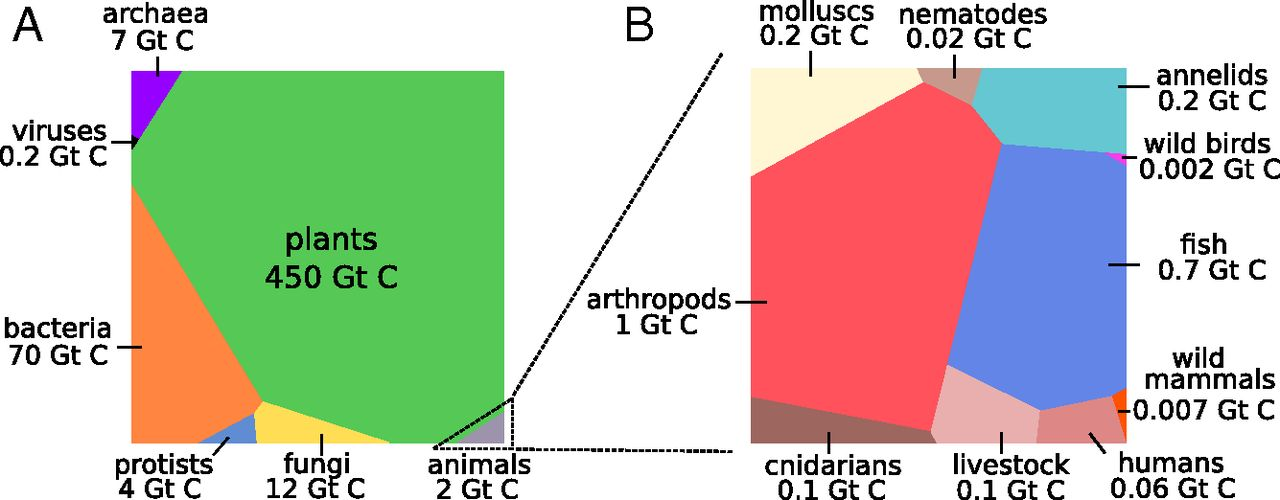
\includegraphics[width=0.7\linewidth]{static/biomass}
    \caption{
    \es{Distribución de la biomasa en el planeta tierra. }%
    }
    \label{fig:biomass}
\end{figure}
En el gráfico de la izquierda podemos ver que la plantas y las bacterias representan el 95\% de la biomasa de la tierra.
En este sentido, la capacidad de adaptación de la información que estas especies almacenan en su sistema genético es varios órdenes de magnitud superior al alcanzado por los seres humanos mediante sus complejos sistemas de información cultural.

\section{Cultura}

La especial integraci\'on de los procesos biol\'ogicos, cognitivos y sociales que permiten a los humanos desarrollar culturas complejas se debió a una coevolución genético-cultural que se desencadenó por el desarrollo previo de la crianza cooperativa~\cite{hrdy2020-emotionallyModern}.
Antes del surgimiento de los humanos \emph{anatómicamente} modernos (masa cerebral actual) y de los humanos \emph{conductualmente} modernos (lenguaje), surgió en África una linaje \emph{emocionalmente} moderno~\cite{hrdy2020-emotionallyModern}.
La forma en la que estos homininos organizaron la crianza produjo un ambiente que favoreció la selección de jóvenes capaces de monitorear y comprender las intenciones de los demás, y de atraer la atención de sus cuidadadores de modo de compartir sus propias necesidades.

% Parrafo

La empatía fue la que permitió el desarrollo del Homo sapiens: la comprensión mutua, la imitación, el lenguaje y finalmente la cultura.
Esta costosa habilidad cognitiva es especialmente eficiente para la adquisición de tradiciones complejas.
Lo que antes debía ser redescubierto una y otra vez mediante costosa experiencia individual, ahora podía ser transmitido a la siguiente generación.
La capacidad de adquirir comportamientos basados en la experiencia de otros sin tener que re-construirlos cada vez por prueba y error conduce un proceso de evolución y acumulativa cultural que permite a las poblaciones humanas adaptarse rápidamente ante cambios bruscos en el ambiente o migraciones a nuevos entornos.

% Parrafo

El surgimiento de la cultura produjo cambios radicales para nuestra especie.
Antes de la transición cultural, estuvimos en grave peligro de extinción, lo que se evidencia en la baja diversidad del genoma humano.
Luego de la transición cultural, en pocos años nuestra especie ocupó todos los nichos ecológicos de la tierra como ningún otro vertebrado terrestre lo había logrado antes.
Esta proeza se logró mediante los sistemas culturales y tecnológico desarrollados por sociedades cazadores-recolectores.
Caminando salimos de África, ocupamos Asia, y de allí Oceanía y las Américas (las flechas del mapa~\ref{fig:agricultura}).
La información transgeneracional fue la que le permitió a estas sociedades simples adaptarse rápidamente a los nuevos desafíos ecológicos.

% Parrafo

El cambio climático ocurrido al inicio del Holoceno (hace 12000 años) propició el desarrollo de la agricultura, que surgió de manera indendiente en los seis grandes sistemas geográficos de la tierra: en la región central de África subsahariana, en Asia occidental, en Asia oriental, en Oceanía norte, en América del norte y en América del sur (las puntos rojos del mapa~\ref{fig:agricultura}).
\begin{figure}[ht!]
    \centering
    \begin{subfigure}[b]{0.6\textwidth}
     \includegraphics[width=\textwidth]{figures/agricultura.pdf}
     \caption{Poblamiento de la tierra y agricultura}
     \label{fig:agricultura}
    \end{subfigure}
%     \begin{subfigure}[b]{0.40\textwidth}
%     \includegraphics[width=\textwidth]{static/polynesia.png} 
%     \caption{Poblamiento del océano Pacífico}
%     \label{fig:polynesia}
%     \end{subfigure}
    \caption{
    El mapa de la figura~\ref{fig:agricultura} es una proyección políedrica de la tierra que conserva los tamaños relativos de los continentes.
    Las felchas indican el poblamiento, desde África a Asia, y de Asia hacia Oceanía y América.
    Los puntos rojos indican surgimiento independiente de agricultura.
    El mapa de la figura~\ref{fig:polynesia}, desarrollado por Thorsby~\cite{thorsby2016-polynesiaAmerica}, muestra el poblamiento de la Polynesia y los contactos con Ámerica evidenciados en el material genéticos. }%
    \label{fig:poblamiento}
\end{figure}
Alrededor de estos puntos se desarrollaron los principales centros poblacionales de la humanidad.
El aumento de la población promovió, a su vez, el desarrollo de nuevas innovaciones tecnológicas y científicas, como la escritura, la matem\'aticas, las ingenier\'ias, la astronomía, las ciencias políticas, entre otras.
Durante el año 1400 el mundo florecía de sociedades "prósperas"~\cite{dussel2004-sistemaMundo}: Aztecas en Ámerica del norte, Incas en Ámerica del sur, Tongas en el Pacífico, Bantúes en África sub-sahariana, los Árabes e Indios en Asia occidental y Chinos en Asia oriental, por mencionar algunos.

% Parrafo

El desarrollo tecnológico de todas estas sociedades fue extraordinario. 
El imperio de Tonga ocupaba hace siglos todo el oc\'eano Pac\'ifico (figura~\ref{fig:polynesia}) con sorprendentes tecnologías de navegación que le habían permitido tener intercambios con América, que se evidencian en el componente genético de los pueblos de la Polynesia~\cite{thorsby2016-polynesiaAmerica, ioannidis2020-polynesiaAmerica}.
En la región Inca se había desarrollado un sistema de intercambios basado en la reciprocidad de trabajo (minka, ayni y mita) que le permitía a las comunidades administrar eficientemente el uso de los bienes comunes y al Estado desarrollar la infrastructura en el vasto territorio montañoso~\cite{murra}.
En la región Azteca se había desarrollado un extenso mercado regional con ciudades de hasta 300.000 habitantes, tres veces la ciudad de Venecia en esa misma época~\cite{www7.uc.cl}. %http://www7.uc.cl/sw_educ/historia/conquista/parte1/html/h54.html
El mundo \'Arabe comerciaba productos desde el Océano Pacífico, en las Filipinas, hasta el Oc\'eano Atl\'antico, en Marruecos, conectando las innovaciones culturales de distintos hemisferios del planeta~\cite{dussel}.
África siempre fue el continente más diverso cultural y genéticamente, pero quizás el centro más innovador en términos científicos y tecnologías haya sido la región de China~\cite{needham2004-generalConclusionsAndReflections}.

% Parrafo

Gracias a estar ubicada en uno de los principales centros geográficos del planeta, China pudo emerger como el corazón del sistema de intercambios planetarios~\cite{pomeranz2000}.
Para el año 1400, China llevaba al menos 2000 de continuidad socio-pol\'itica, y 900 a\~nos de un estado meritocr\'atico en el cual sus miembros eran elegidos a trav\'es de concurso público (examen imperial).
Inventa el acero en el siglo segundo, el papel en el siglo sexto, la imprenta en el siglo octavo, el papel moneda en el noveno, la br\'ujula en el onceavo.
Desarrolla infraestructuras como el canal navegable \emph{Da Yunhe} de más de 1700 kilómetros para conectar la ciudad de Pekín con otras ciudades importantes, y la famosa muralla que en total superó los 20000km de longitud.
China ya era de hecho el principal proveedor comercial del resto del mundo.
No parecían necesitar nada más afuera de sus fronteras.
Es así como a pesar de que desarrolla la flota más grand de la historia, dirigidas por Zheng He (1405-1433), el Gobierno Chino decide cerrarse fronteras adentro dándolas por finalizadas por completo.

% Parrafo

Así como la integración favorece los proceso de innovación y acumulación cultural, el asilamiento induce pérdidas masivas de información cultural.
Un ejemplo de aislamiento total bien documentado ocurre con la separación de Tasmania del continente Australiano por la subida del nivel del mar ocurrida a comienzos del Holonceno.
La evidencia arqueológica y etnohistórica indica que desde el principio del Holoceno las sociedades de Tasmania perdieron gran parte de su cultura tecnológica.
La principal hipótesis sugiere que la reducción del tamaño efectivo de la población (\emph{effective population size}) fue la causa más importante de estas pérdidas culturales~\cite{henrich2004-demographyAndCulturalEvolution}.

\begin{figure}[ht!]     
  \centering 
  \begin{subfigure}[c]{0.45\textwidth}
    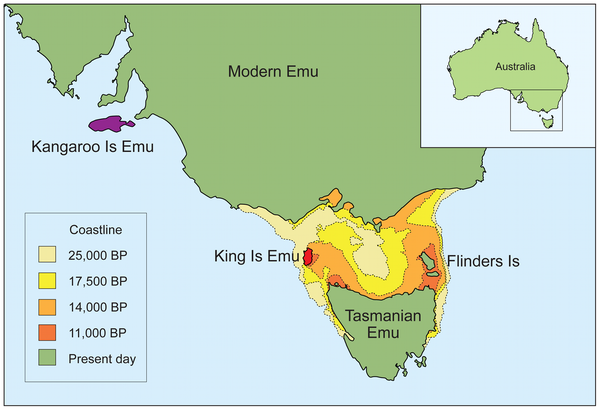
\includegraphics[width=\textwidth]{static/tasmania.png} 
    \caption{Tasmania}
    \label{fig:tasmania}
  \end{subfigure}
  \begin{subfigure}[c]{0.45\textwidth}
    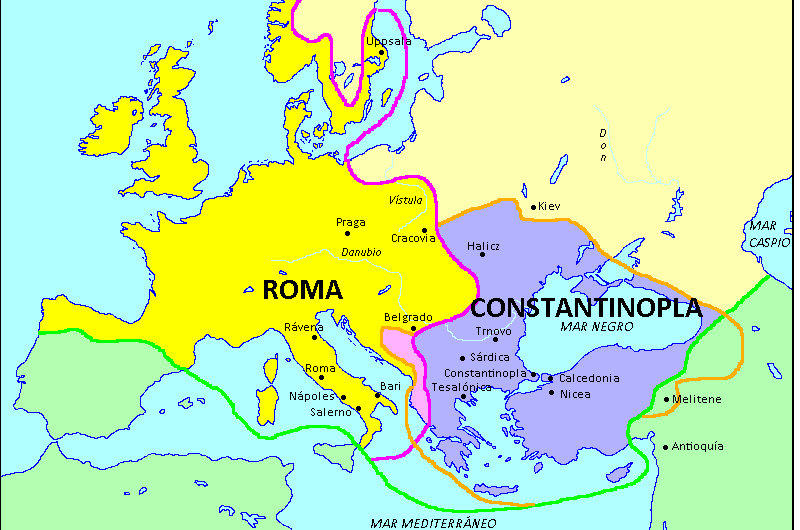
\includegraphics[width=\textwidth]{static/cisma.png} 
    \caption{Edad media}
    \label{fig:cisma}
  \end{subfigure}
  \caption{Aislamiento}
  \label{fig:aislamiento}
\end{figure}

Un caso de asilamiento parcial ocurre en Europa occidental.
Arrinconada ya en el lejano occidente por el fr\'io polar y la falta de tecnolog\'ias de navegaci\'on del Atlántico, Europa occidental comienza en el siglo octavo a quedar paulatinamente aislada del ``sistema mundo'' por la expansión Árabe al sur y por la serie cismas con el Imperio Bizantino al Oeste~\cite{Dussel}.
Esa etapa de aislamiento coincide con el proceso de perdida masivas de información cultural y de degradación de las condiciones socio-económicas conocido como ``edad media'', un proceso que sólo ocurre en Europa occidental.
Si no era posible recuperar el acceso al sistema mundo por el Oriente a través de las cruzadas, la única opci\'on que quedaba era explorar los mares del Este.

% Parrafo

Producto de la pésima situación socio-económica de la ``edad media'', apenas Europa occidental descubre cómo navegar el Atlántico, comienza un masivo proceso migratorio.
La coincidencia de un conjunto de eventos puso a esta sociedad, históricamente marginal, en una situación de privilegio mundial.
Un siglo antes, China hab\'ia incorporado la plata como monedad oficial, la que ya estaba siendo utilizada como moneda de cambio en todo el mundo Árabe~\cite{pomeranz2000-divergence, pomeranz2018-tradeCreated}.
En América del sur el estado incaico que estaba organizado en base a un sistema de intercamios no monetarios en una región montañosa rica en minerales precisosos.
Además de la buena predisposición con la que los exploradores reportan haber sido recibidos por los habitantes Americanos, la llegada de masiva de emigrantes feudales produjo una serie de pandemias que redujeron la población local en por lo menos 60\% entre los años 1500 y el 1600~\cite{koch2019-europeanArrival}.

% Parrafo

Cuando 1546 los exploradores descubren la montaña de plata de Potosí, en el centro del sistema estatal incaico, la Europa feudal queda inmediatamente en una posición de privilegio en todo el mundo afro-euro-asiático.
Mediante la captura del sistema administrativo incaico (golpe de estado) los impuestos que antes antes se destinaban al desarrollo de la infraestructura, comienza a ser utilizado para extraer la plata, un mineral sin interés por los nativos.
En poco tiempo la plata Árabe queda devaluada ante la inmensa cantidad de plata que llagaba de América.
Así es que 25 años después, en 1571, Europa occidental rompe en el Meditarraneo el asilamiento sufrido durante la edad media (batalla de Lepanto).
La integración privilegiada al sistema mundo inicia un proceso rápido de acumulación cultural basado en las tecnologías extranjeras.
La plata de América fluye en todas las direcciones, principalmente en dirección a China.

\begin{figure}[ht!]     
  \centering 
  \begin{subfigure}[b]{0.48\textwidth}
    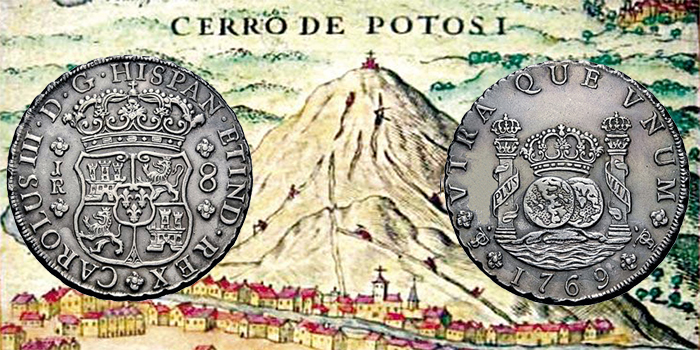
\includegraphics[width=\textwidth]{static/plata-potosi} 
    \caption{Plata}
    \label{fig:potosi}
  \end{subfigure}
   \ \ 
  \begin{subfigure}[b]{0.47\textwidth}
    \includegraphics[width=\textwidth]{figures/china.pdf} 
   \caption{Opio}
    \label{fig:china-pop}
  \end{subfigure}
  \caption{La plata y el opio como las llaves de la integración privilegiada de la Europa occidental en el sistema mundo.}
  \label{fig:integracion}
\end{figure}

Durante 250 años la plata americana sirvió para muchas cosas, pero principalmente para comprar productos chinos y financiar la primera industrialización británica con tecnología China.
Europa consumía productos asiáticos, pero exportaba muy poco a Asia.
El comercio internacional de opio comenzó en el 1700 como respuesta a una crisis del comercio internacional europeo, especialmente británico.
El opio, un producto lujoso utilizado en China como medicina (raramente como estupefaciente), fue prohibida por los emperadores chinos en 1729, que por su abundancia hacía crecer lentamente la cantidad de adictos.
Las consecuencias fueron más graves cuando en 1818 se desarrolla una mezcla de opio más barata y potente.

% Parrafo

Mediante el narcotráfico Europa occidental consigue por primera vez, en el siglo 19, revertir el déficit comercial que siempre tuvo con China, desde los tiempos del imperio romano.
El número de adictos llegó a ser lo suficientemente alarmante, y en 1839 China comete el error de declarar la guerra al narco-estado británico en su propio territorio.
Los resultados fueron terribles.
Los chinos no sólo no pudieron impedir el ingreso de la droga, perdieron también su autonomía arancelaria, el derecho a someter a los residentes extranjeros a la ley china.
Expuesta a su debilidad militar, China sufrió un siglo calamitoso de agresiones extranjeras, desorden interno y guerra civil, que produjo una caída de 1/5 de su población (figura~\ref{fig:china-pop}).

% Parrafo

Luego de la derrota de China por parte del narco-estado británico, se establece finalmente la hegemonía de Europa occidenta en el sistema mundo y se profundiza el proceso de colonización en todo el mundo. % que hasta el momento estaba limitado estatales de América continental estaba limitada a puertos e islas.
En 1850 comienza la colonización de África continental y de los extensos territorios americanos que todavía seguían a manos de comunidades locales.
Comienza la era de los genocidios.
Todos los conocimientos que la sociedad colonial va incorporando del resto de comunidades del mundo se les borra su verdadero origen histórico y se las enaltecen como surgimientos espontaneos internos.
Es una nueva era de avances científicos y tecnológicos, pero por otro es la era de pérdida de diversidad cultural.
En todas las partes del globo, los exploradores y etnógrafos fueron documentando la perdida de cultural debida al avance del frente colonial-moderno, estatal o privado, sobre las autonomías locales.

\section{Ciencia}

A pesar de todos los avances científicos, la ciencia metropolitana moderna no fue capaz de compensar la perdida de los conocimientos milenarios acumulados por las comunidades autónomas locales.
Los estudios comparados indican que las únicas instituciones capaces de administrar a largo plazo los bienes comunes, nunca fueron ni estatales ni privadas, son de tipo comunitarias histórico arraigo local~\cite{ostrom2009,ostrom1990}.
La masiva pérdida de diversidad cultural trajo como consecuencia la masiva pérdida de biodiversidad actual, una crisis ecológica sin precedentes.
Los conocimientos milenarios y sus instituciones adaptadas ecológicamente se pierden definitivamente en unas pocas generaciones.
En un mundo de comunidades debilitadas, la pedagogía de la crueldad fedual-colonial-moderna logra introducir la cosmovisión individualista e instrumental de nuestro tiempo: la naturaleza como cosa, las personas como cosas.
%La intervención irracional de un grupo de humanos sobre el sistema ecológico, reservorio del principal conocimiento empírico para la vida, es la analogía más acabada de la imposición de la mentira sobre la verdad.

\begin{figure}[ht!]
    \centering
    \begin{subfigure}[b]{0.48\textwidth}
    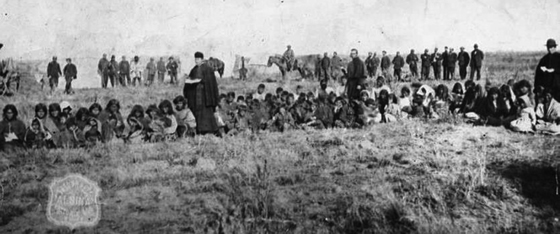
\includegraphics[width=\linewidth]{static/genocidio_patagonia}
    \caption{Genoetnocidios}
    \label{fig:genocidio_patagonia}
    \end{subfigure}
    \begin{subfigure}[b]{0.47\textwidth}
    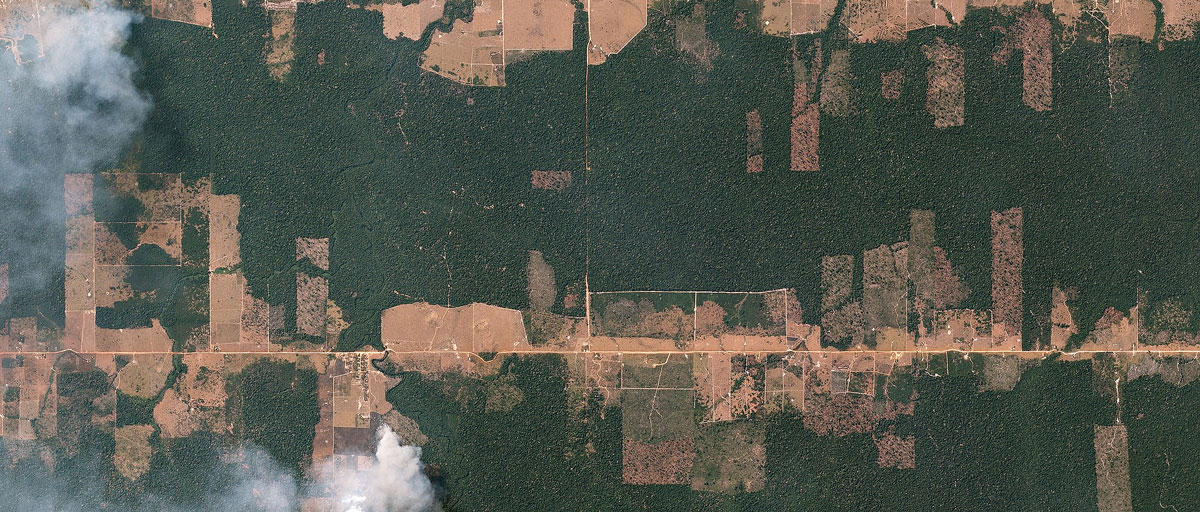
\includegraphics[width=\linewidth]{static/deforestation-brazil}
    \caption{Crisis ecológica}
    \label{fig:deforestation-brazil}
    \end{subfigure}
    \caption{
    La masiva pérdida de diversidad cultural trajo como consecuencia la masiva pérdida de biodiversidad actual, una crisis ecológica sin precedentes.
    }
    \label{fig:cultural-lose}
\end{figure}

La misma naturaleza multiplicativa de los procesos evolutivos que había ofrecido una ventaja física para la agregación cooperativa de las formas de vida, favoreció también la aparición de instituciones culturales basadas en la reciprocidad.
La supervivenvia de una comunidad depende del renovación permanente de los vínculos interpersonales, de la salud de su tejido comunitario.
Lo que identifica a este sujeto colectivo, los pueblos, es la autopercepción por parte de sus miembros de compartir una historia común, que viene de un pasado y se dirige a un futuro, aun a través de situaciones de disenso interno y conflictividad~\cite{segato2016-guerraContraLasMujeres}.
La experiencia acumulada a través de las generaciones por las más diversas comunidades del mundo condujo, de forma independiente, al desarrollo de tecnologías de sociabilidad sorprendentemente similares entre sí.
En todas ellas se pueden reconocer al menos dos mecanismos que cumplen la función de re-ciclar los v\'inculos interprersonales: los ritos festivos y los ritos coercitivos~\cite{segato2016-guerraContraLasMujeres}.

% Parrafo

Los ritos coercitivos no son otra cosa que ceremonias para la reactivación de flujos de intercambios rotos previamente por conflictos entre partes.
Están orientados el restablecimiento de los vínculos mediante los mecanismos de ``reparación'', ``conciliación'' y ``ayuda'' \cite{zaffaroni2013-cuestionCriminal}, haciendo uso de los tres tipos de intercambios posibles entre partes: 
($\rightarrow$) el acto en el cual el acusado (o sus representantes) da algo al acusante (o sus representantes);
($\leftrightarrow$) el acto en el cual el acusado y acusante (o sus representantes) dan y reciben mutuamente;
($\leftarrow$) el acto en el cual el acusado (o sus representantes) recibe algo del acusante (o sus representantes).
La expulsión del agresor de la comunidad sólo se prevee en casos extremadamente excepcionales, pues el primer derecho de sus miembros es el derecho a la comunidad \cite{segato}.

% Parrafo

Los estudios comparativos sobre instituciones administradores de bienes comunes concluyen que su capacidad de supervivencia a largo plazo está asociada con la presencia de las siguientes caracterísiticas:\vspace{-0.1cm}
\begin{description}\setlength\itemsep{-0.1cm}
 \item[1. Identidad comunitaria y territorial:] el reconocimiento de miembros y del sistema ecológico específico sobre el cual se ejerce la jurisdicción.
 \item[2. Instituciones adaptación social y ecológica:] Las normas son compatibles con las condiciones sociales y medioambientales locales.
 \item[3. Deliberación comunitaria:] La mayoría de los individuos involucrados en el sistema ecológico están autorizados a participar en la elaboración y modificación de sus normas.\setlength\itemsep{-0.1cm}
 \item[4. Conocimiento experto local:] La supervisión de los compartamientos de las personas el sistema ecológico está a cargo de los mismos miembros.\setlength\itemsep{-0.1cm}
 \item[5. Garantías de derechos comunitatrias:] Las sanciones son graduales, comienzan siendo muy bajas, y sólo raramente se decide la expulsión de la comunidad porque el primer derecho es formar parte de una comunidad.
 \item[6. Ritos festivos y coercitivos:] ceremonias de intercambio para el restablecimiento de los vínculos comunitarios mediante los mecanismos de ``reparación'', ``conciliación'' y ``ayuda''.
 \item[7. Autonomía comunitaria:] el reconocimiento de las comunidades vecinas a establecer sus propias normas.
 \item[8. Relaciones intercomunitarias] cuando un recurso de uso común está conectado a un sistema socioecológico más amplio, las actividades se organizan en múltiples capas anidadas.
\end{description}

% Parrafo

Europa occidental también estuvo constituida por este tipo de comunidades.
Si bien el imperio romano eliminó una parte importante de este paisaje cultural, no alcanzó a eliminarlo por completo.
Los ``bárbaros'' justamente eran comunidades autónomas establecidas en la parte norte de Europa occidental, que persistieron luego de la caída del imperio romano de occidente.
Pero la ``edad media'' fue una anomalía en la historia de la humanidad.
En la etapa de aislamiento comenzó a ganar terreno al interior de la sociedad feudal el criterio de autoridad (sexual, militar, académica, moral) como fundamento del ``saber auténtico''.
Las instituciones heredadas del imperio romano de occidente, en cabeza de la iglesia católica romana, comenzaron a competir con las comunidades indígenas locales y a producir una conjunto de novedosas tecnologías de colonización~\cite{zaffaroni2013-cuestionCriminal}. 

% Parrafo

Una de las primeras y más importante tecnologías de colonización que desarrolla la iglesia católica romana es la regulación de las relaciones comunitaria de reproducción de forma más detallada que la propiedad.
Esta acción proscribe el rol político que las mujeres desempeñan en la administración del espacio doméstico comunitario, interviniendo en el funcionamiento de sus tecnologías de sociabilidad.
Se debilita así el arraigo comunitario, facilitando la captación de población desertora para actividades militares.
\begin{figure}[ht!]
    \centering
    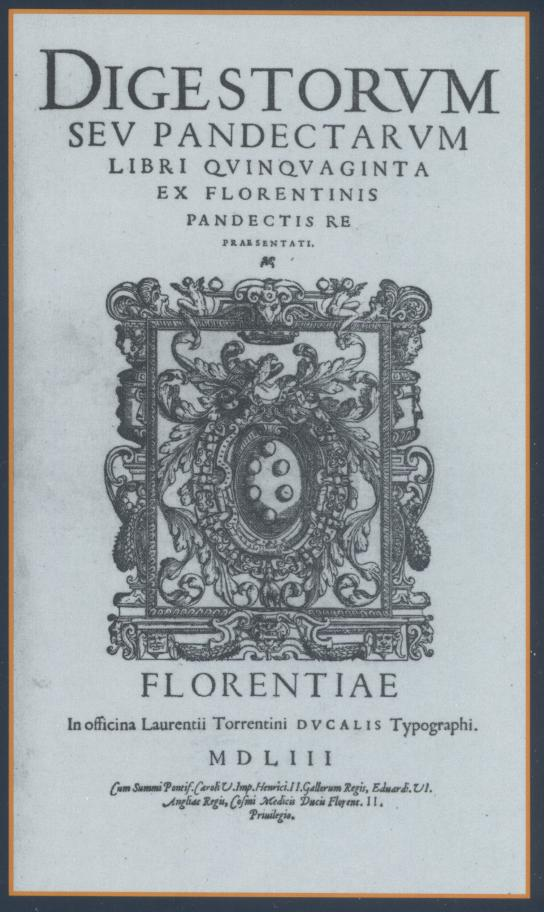
\includegraphics[width=0.18\linewidth]{static/digesto1553.jpg}
    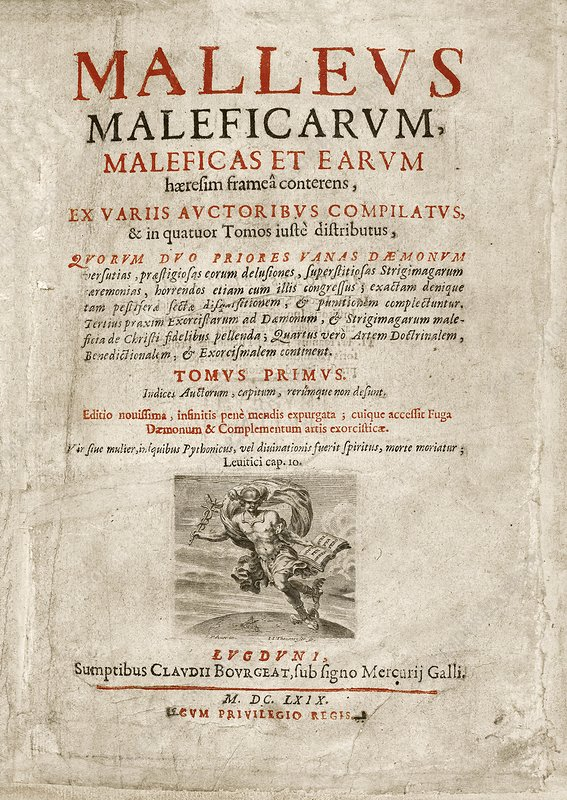
\includegraphics[width=0.213\linewidth]{static/malleus.jpeg}
    \caption{El criterio de autoridad como fundamento del ``saber auténtico'' y la guerra contra las mujeres como tecnología de colonización. %La proscripción de las tecnología de sociabilidad comunitaria, acción política del espacio doméstico administrada principalmente por las mujeres, debilita el arraigo comunitario facilitando la capatación de población desertora para actividades militares.
    }
    \label{fig:malleus}
\end{figure}
El poder punitivo se fue extendiendo y un nuevo sistema penal re-nació de los llamados \emph{libris terribilis} del Digesto, antiguas leyes romanas recolectadas por encargo del emperador Justiniano de Constantinopla pero re-interpretadas en occidente de modo de liberar al poder punitivo de todo límite.
En esta etapa, el sujeto masculino se torna modelo de lo humano y de todo cuanto sea dotado de politicidad, interés general y valor universal, y el espacio de las mujeres se transforma en margen y resto de la política.
La guerra contra las mujeres se formaliza definitivamente con la publicación del \emph{Malleus maleficarum} en 1484, que es el segundo best seller de la modernidad después de la Biblia durante los siguientes 200 años.

% Parrafo

Sólo después de que la sociedad feudal adquiere una posición de privilegio  en el sistema mundo, comienza al interior de esta sociedad, ahora colonial-moderna, un nuevo debate sobre las fuentes de validación del conocimiento.
En esta etapa el criterio de experiencia personal comenzó ganar terreno como fundamento del ``saber auténtico'' sobre los criterios de autoridad.
Esto abrió un debate entre posiciones que parecían irreconciliables. 
Algunos lo entendieron la experiencia como ``evidencia intelectual'' (racionalistas) y otros como ``evidencia sensible'' (empiristas).
Sin embargo, de ambos lados existió un consenso de que el nuevo criterio, que servía para democratizar el conocimiento al interior de la sociedad feudal, estaba reservado para uso exclusivo de sus miembros varones.

% Parrafo

El argumento de la superioridad moral, que es utilizado durante toda la modernidad hasta el presente, lo desarrolla por primera vez Ginés de Sepúlveda cuatro años después del descubrimiento de la plata de Potosí, en 1550.
\begin{quotation}
 Será siempre justo y conforme al derecho natural que tales gentes [bárbaras] se sometan al imperio de príncipes y naciones más cultas y humanas, para que por sus virtudes y la prudencia de sus leyes, depongan la barbarie y se reduzcan a vida más humana y al culto de la virtud [...] Y si rechazan tal imperio se les puede imponer por medio de las armas, y tal guerra será justa según el derecho natural lo declara [...] En suma: es justo, conveniente y conforme a la ley natural que los varones probos, inteligentes, virtuosos y humanos dominen sobre todos los que no tienen estas cualidades~\cite{GinesdeSepulveda1967p87}.
\end{quotation}
Este idea no se ve afectada por el argumento que propone Kant, conocido como el imperativo categórico, de que la validez del conocimiento radica en el reconocimiento mututo,
\begin{quotation}
Obra de tal modo que la máxima de tu voluntad pueda valer siempre al mismo tiempo como principio de una legislación universal \cite{Kant2003:28}.
\end{quotation}
El mismo Kant no percibe una contradicción cuando unos parrafos más adelante el mismo considera que las razas americanas son incapaces de toda cultura y que las razas negras pueden ser educadas pero sólo como sirvientes y esclavos.
No hay contradicción porque el concepto colonial-moderna de ``universalidad'' nace limitado.
Mujeres, extranjeros, animales y sistemas ecológicos completos participan sólo como objetos de los varones-blancos, estos últimos únicos sujetos con valor universal.
La sociedad colonial-moderna, y su ciencia, repite la estructura verticalista y punitivista de la sociedad feudal, ahora con alcance global gracias a la plata Americana.

% Parrafo

Todos los conocimientos que la nueva sociedad colonial-moderna va incorporando de todos los rincones del mundo, se les borra su verdadero origen histórico y se las enaltecen como surgimientos espontaneos internos.
Recién en 1800 Hegel propone por primera vez una periodización histórica que coloca a Europa occidental, que había sido históricamente marginal del sistema mundo, como centro y fin de la Historia Universal: \emph{antigüedad} - \emph{edad media} - \emph{modernidad}~\cite{dussel2007}. 
El mito eurocéntrico proyecta a la Europa feudal en la cultura griega y judeo-cristiana (ambos fenómenos de origen oriental) con pretensión de explicación histórico-mundial: ``la historia universal va del Oriente al Occidente; Europa es el centro absoluto de la historia universal'' dice Hegel~\cite{hegel}.

% \begin{figure}[ht!]
%     \centering
%     \begin{subfigure}[b]{0.15\textwidth}
%     \centering
%     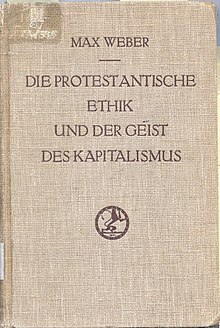
\includegraphics[width=\linewidth]{static/weber}
%     \caption{Weber}
%     \label{}
%     \end{subfigure}
%     \begin{subfigure}[b]{0.15\textwidth}
%     \centering
%     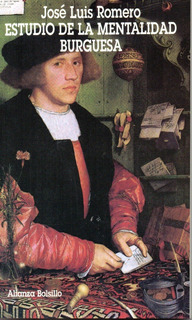
\includegraphics[width=0.9\linewidth]{static/romero}
%     \caption{Romero}
%     \label{}
%     \end{subfigure}
%     \begin{subfigure}[b]{0.15\textwidth}
%     \centering
%     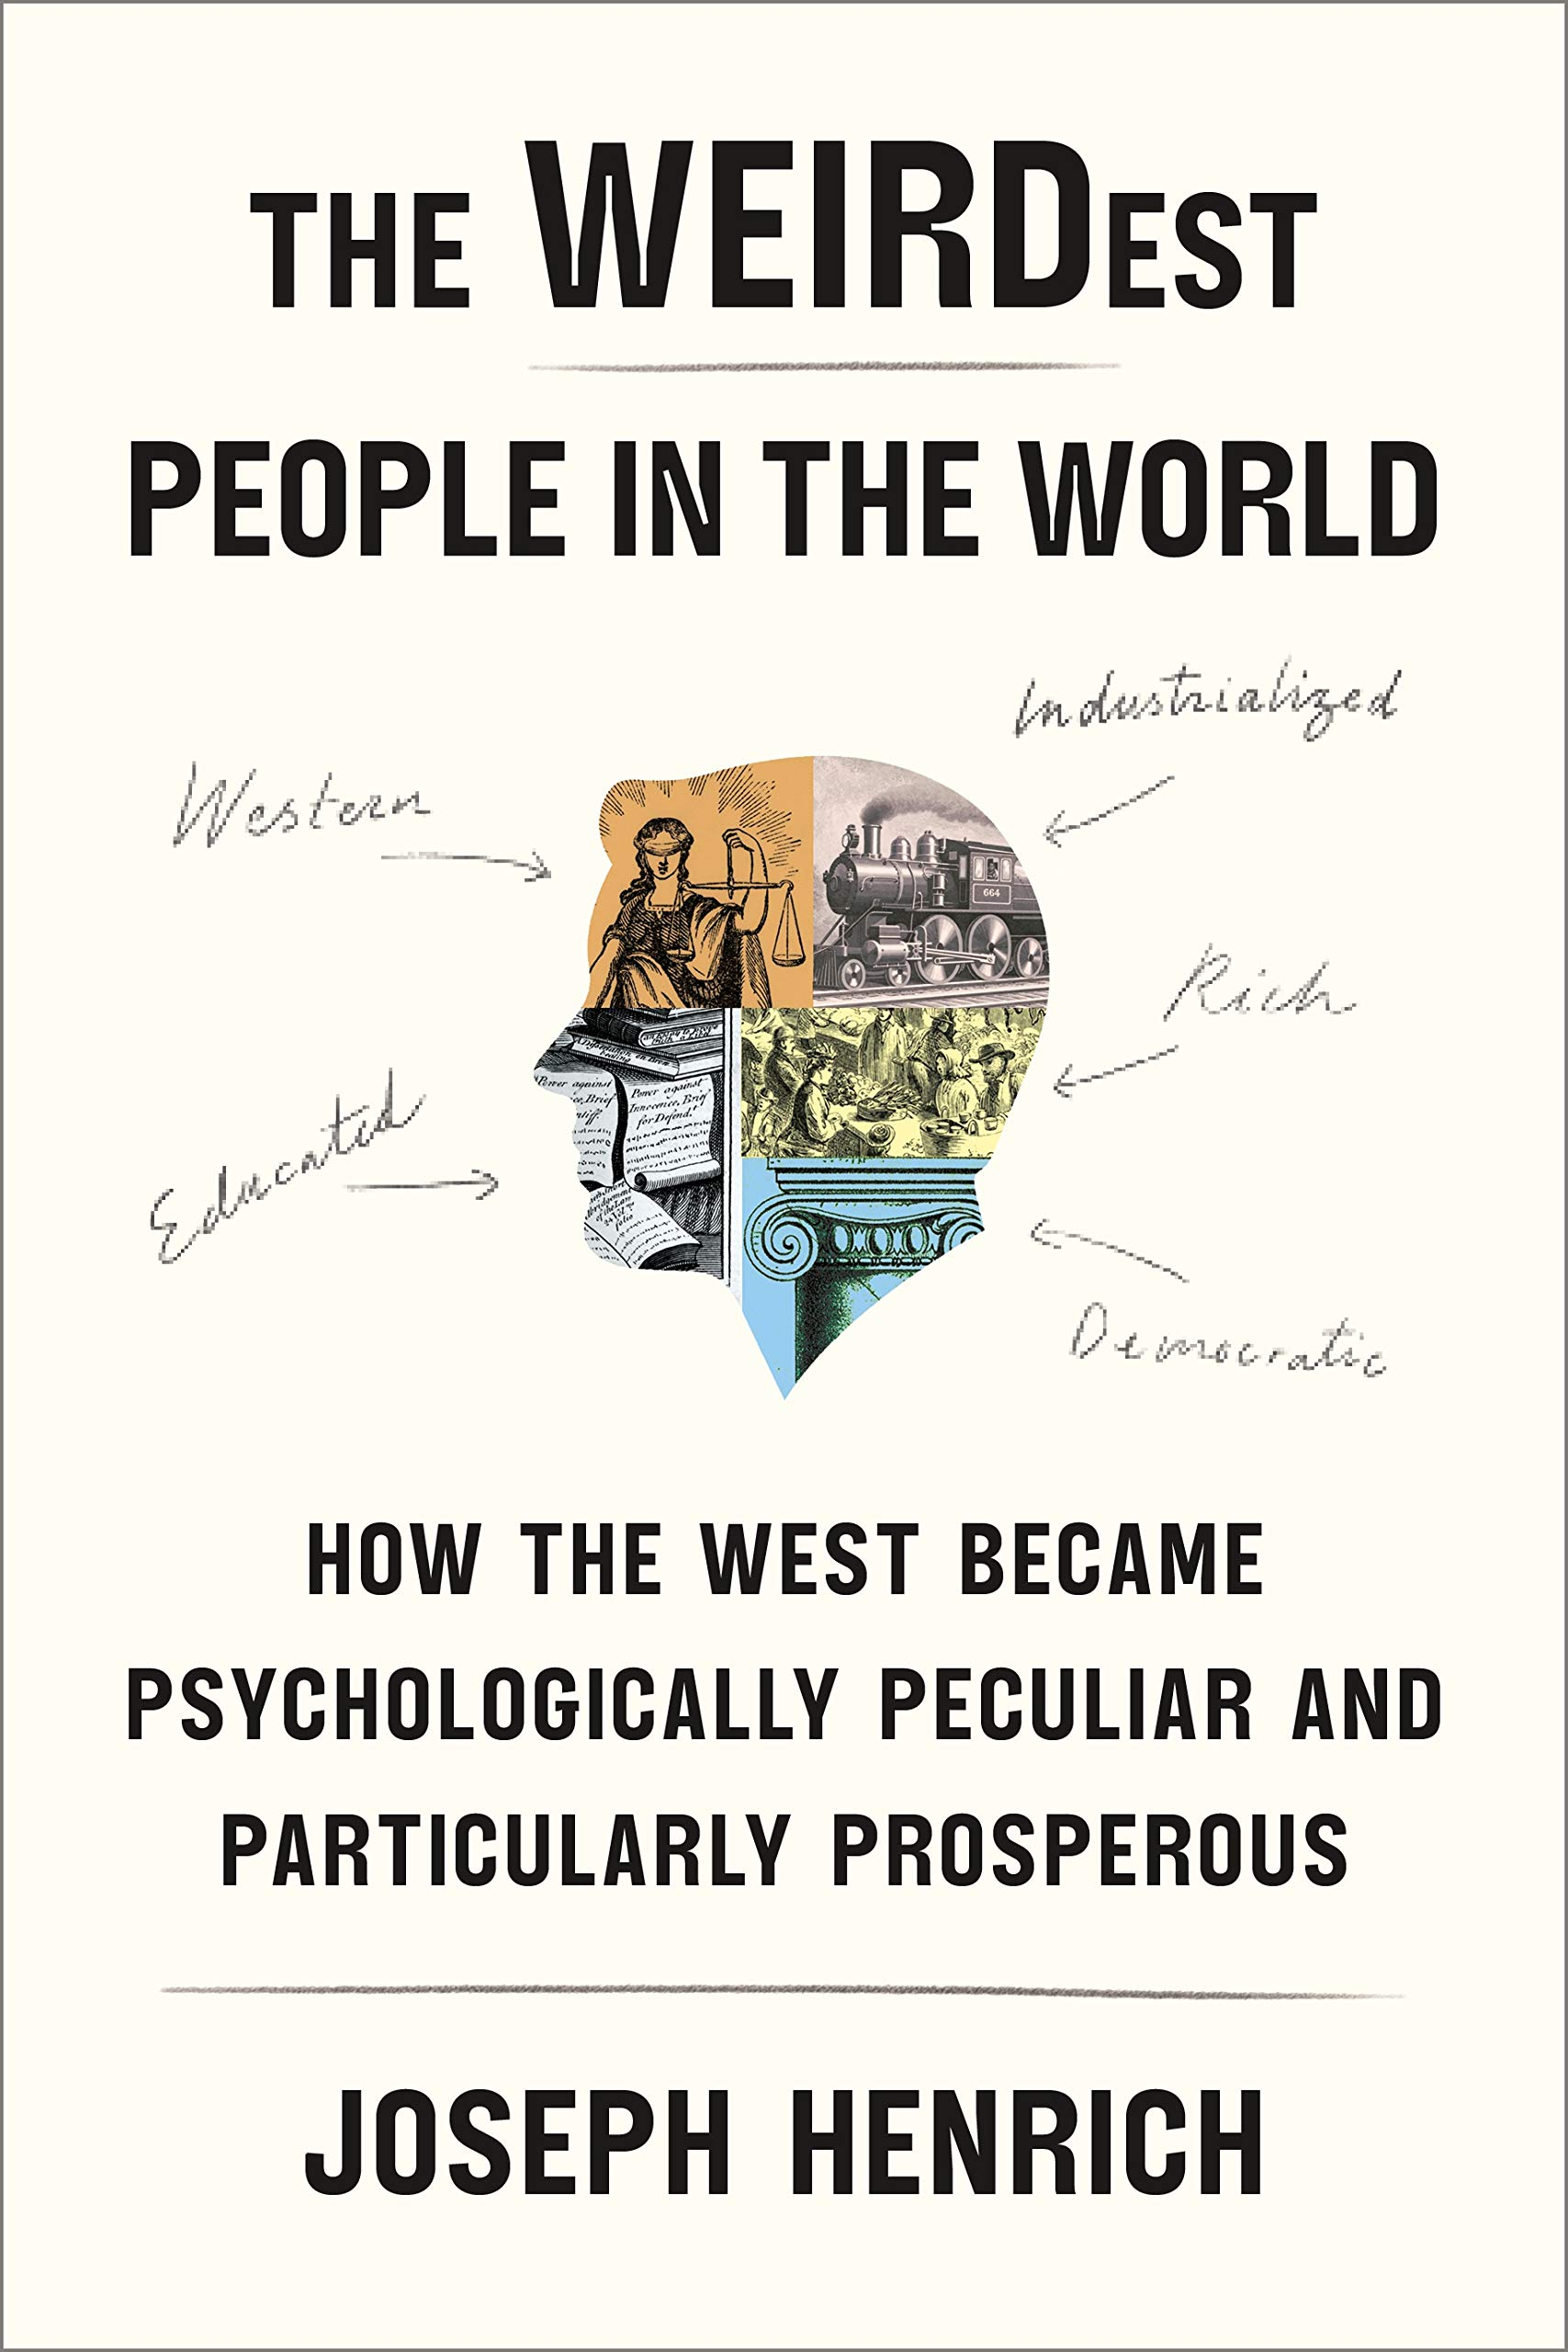
\includegraphics[width=1\linewidth]{static/henrich}
%     \caption{Henrich}
%     \label{}
%     \end{subfigure}
%     \caption{Mito eurocéntrico}
%     \label{fig:mito}
% \end{figure}

Este relato falso de la historia está vigente todavía hoy en la principales univerisidades del mundo occidental, desde Harvard a la Universidas de Buenos Aires, tanto en universidades de África, el mundo Árabe, India y Asia.
Desde Hegel hasta la fecha, las explicaciones eurocéntricas intentan explicar la proposperidad actual de occidente a través de una causa interna: el ``espíritu protestante'' de Weber \cite{weber}, la ``mentalidad burguesa'' de Romero \cite{romero}, o más recientemente el ``sistema de parentezco''\cite{henrich} de Henrich.
La paradoja que no puede responder el relato eurocéntricos es cómo una sociedad sumida en un proceso de involución cultural, como la sociedad feudal de la ``edad media'', pudo generar de repenten el proceso de desarrollo científico y técnico de la modernidad.

% Parrafo

Ninguna de las explicaciones eurocéntricas incorpora en su análisis la situación de aislamiento que sufre Europa occidental en la etapa previa ni la posterior situación de integración privilegiada en el sistema mundo.
Incluso Needham, el británico que recopiló la monumental historia científica y técnica de China, reconoce que comenzó a estudiar el tema motivado por responder la pregunta de por qué sólo Europa occidental había logrado el avance científico.
\begin{quotation}
When I first formed the idea, about 1938, (...) I regarded the essential problem as that of why modern science had not developed in Chinese civilisation (or Indian or Islamic) but only in that of Europe~\cite{needham2004-generalConclusionsAndReflections}.%
\end{quotation}
Luego de 60 años de investigaciones, Needham se ve obligado inviertir la pregunta.
\begin{quotation}
Why, between the -1th century and the 15th century, was Chinese civilisation much \emph{more} efficient than occidental in gaining natural knowledge and in applying it to practical human needs?~\cite{needham2004-generalConclusionsAndReflections}
\end{quotation}

% Parrafo

La Europa feudal no se había despertando del impacto de su invasión colonial cuando ya en 1514 Bartolomé de la Casas inicia desde América la advertencia de los efectos negativos de la integración basada en la dominación que promovían los primeros migrantes feudales.
En su crítica Bartolomé:
a) refuta la pretensión de superioridad de la cultura occidental sobre las las culturas indígenas;
b) diferencia entre otorgar al otro (al indio) pretensión universal de verdad, sin renunciar a la pretensión de predicar a favor la propia cultura cristiana;
c) y demuestra la falsedad del argumento usado para justificar la intervención en las autonomías locales, basado en el supuesto ``remedio a las injusticias internas'', en tanto esa intervenciones producían peores efectos sobre las poblaciones intervenidas.

% Parrafo

En efecto, luego de cinco siglos podemos ratificar los efecto negativos del criterio de autoridad feudal globalizado durante la colonial-modernidad: la masiva perdida de biodiversidad que está en curso en la actualidad es el producto de la ciencia y técnica moderna.
La defensa de la diversidad cultural no se sustenta en argumentos relativistas, que reclaman el derecho de los pueblos a mantener su patrimonio cultural ancenstral.
El derecho a las autonomías comunitarias se sustenta en el hecho práctico de que el conocimiento cultural ecológicamente adaptado sólo evoluciona a través de la experiencia histórica que acumulan los pueblos~\cite{Rita}.

\begin{figure}[ht!]
    \centering
    \begin{subfigure}[b]{0.45\textwidth}
    \centering
    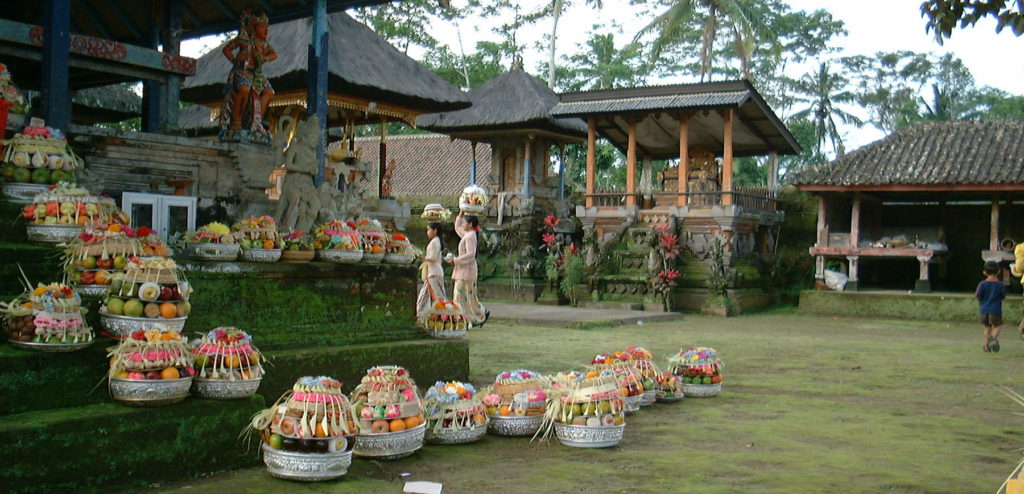
\includegraphics[width=\linewidth]{static/bali-offerings}
    \caption{Canang sari}
    \label{}
    \end{subfigure}
    \begin{subfigure}[b]{0.33\textwidth}
    \centering
    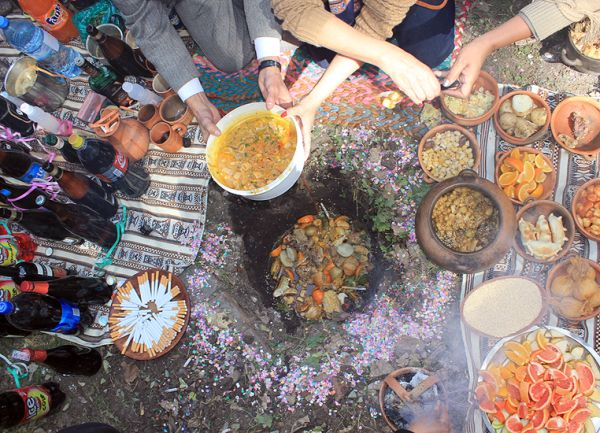
\includegraphics[width=\linewidth]{static/pachamama}
    \caption{Pachamama}
    \label{}
    \end{subfigure}
    \caption{La Madre Naturaleza como sujeto de derecho.}
    \label{fig:mito}
\end{figure}

El reconocmiento mutuo, que estuvo en la base de la evolución de nuestra especie, debe adquirir una universalidad plena para que valga como fundamento del conocimiento, que ni la propuesta parcial de Kant ni su cultura colonial ha sido capaz de alcanzar.
Debemos obrar de una vez por todas ``de tal modo que la máxima de nuestra voluntad pueda valer siempre al mismo tiempo como principio de una legislación universal'', reconociendo esta vez como sujetos con valor universal a la diversidad toda: el estatus social y político que las mujeres encabezan en el espacio comunitario, el reconocimiento de las autonomía comunitarias, pero también el derechos de la madre tierra (\emph{pachamama}) de no ver interrumpido sus procesos ecológicos sin justa causa: lo mínimo necesario para el buen vivir (\emph{suma kausay}).


\newpage

\section{Funciones}

\section{Honestidad}

\section{Base empírica}

\section{Selección de modelos}

\section{Conclusiones}


\chapter{Modelos de estimación de habilidad (TTT)}

\chapter{Sistema de estimación para el juego Go (AAGo).}

\chapter{Efecto de los equipos sobre el aprendizaje (faithfull-sinergia)}

\chapter{Efecto de la topología sobre el aprendizaje.}


\end{document}
